% !TEX root = ../main.tex

\chapter{颗粒介质的剪切响应}

\section{引言}

对于颗粒间非固结的颗粒介质,其具有一定的抗剪切作用。然而颗粒间的接触及其产生的作用力很容易因为外部剪切作用导致的颗粒重排而发生变化,因此与寻常固体的应力-应变关系存在着差异。颗粒介质内部存在着不同强度的力链,其中强力链承担了介质中绝大部分的应力成分;当强力链上的颗粒成员受到外部激励而发生相对位移时,介质的应力就可能会发生较大的变化,这也是颗粒介质的奇异力学响应来源。

在第一章中我们已经提到过,等大硬球颗粒堆积存在着两种随机堆积的体积分数极限,即随机密集堆积(RCP)与随机松散堆积(RLP),这两种堆积状态的颗粒介质对于外部剪切的响应并不相同;而在密堆积中,颗粒介质也会因为所受的剪切法向应力不同而产生不同的力学响应表象。


\subsection{STZ 理论}

Shear Transformation Zone(STZ)认为,像颗粒固体这类非晶体材料在受到剪切时,会同时出现弹性形变和塑性形变,后者则是因为颗粒间发生了不可逆的相对位移。在颗粒介质受到剪切时,我们关注其中接触结构发生变化的区域。令塑性形变量为 $\varepsilon_{\text{pl}}$(pl=plastic),颗粒介质中的空隙体积为 $V_{f}$(f=free,即自由体积)。假定在剪切转变区域中存在两种不同的状态,使用 + 和 - 来对其进行表述,并引入 $n_{\mp}$ 来表示处于状态 $\mp$ 的数密度。在上述约定下,Langer 推导出了空隙体积变化率方程\cite{PhysRevE.64.011504}:

\begin{equation}
  \dot{V_{f}} = -E_{1}\cdot{\ee}^{-\frac{V_{1}}{V_{f}}} + A_{V}|\sigma\dot{\varepsilon}_{\text{pl}}|,
\end{equation}

其中 $E_{1}$、$A_{V}$ 是常数,$V_{1}$ 表示的是受剪切区域刚放生变化时的自由体积大小(也被称作临界自由体积),$\sigma$ 表示介质所受的偏应力。$\varepsilon_{\text{pl}}$ 定义如上,且存在关系

\begin{align}
  \dot{\varepsilon}_{\text{pl}} = E_{0}{\ee}^{-\frac{V_{0}}{V_{f}}}\left[\Lambda\sinh{(\sigma)} - \Delta\cosh{(\sigma)}\right],\\
  \Lambda = \frac{n_{-} + n_{+}}{n_{\infty}},\quad\Delta = \frac{n_{-} - n_{+}}{n_{\infty}}.
\end{align}

其中 $n_{\infty}$ 是 $(n_{-} + n_{+})$ 在稳定平衡态下的值。对于 $\Lambda$ 和 $\Delta$,其行为被描述为

\begin{align}
  \dot{\Delta} &= \frac{1}{\varepsilon_{0}}\left(\dot{\varepsilon}_{\text{pl}} - \gamma|\sigma\dot{\varepsilon}_{\text{pl}}|\Delta\right),\\
  \dot{\Lambda} &= \frac{\gamma}{\varepsilon_{0}}\left|\sigma\dot{\varepsilon}_{\text{pl}}\right|(1-\Lambda)
\end{align}

使用 STZ 理论,可以描述颗粒介质在受剪切时出现的蠕变和滞滑现象。

\section{实验装置}

目前剪切装置和声学装置的耦合尚不成熟,因此只简要介绍有关于剪切装置的部分。图~\ref{fig:apparatus_2} 展示了剪切实验中的各部件。

\begin{figure}[!htp]
    \centering
    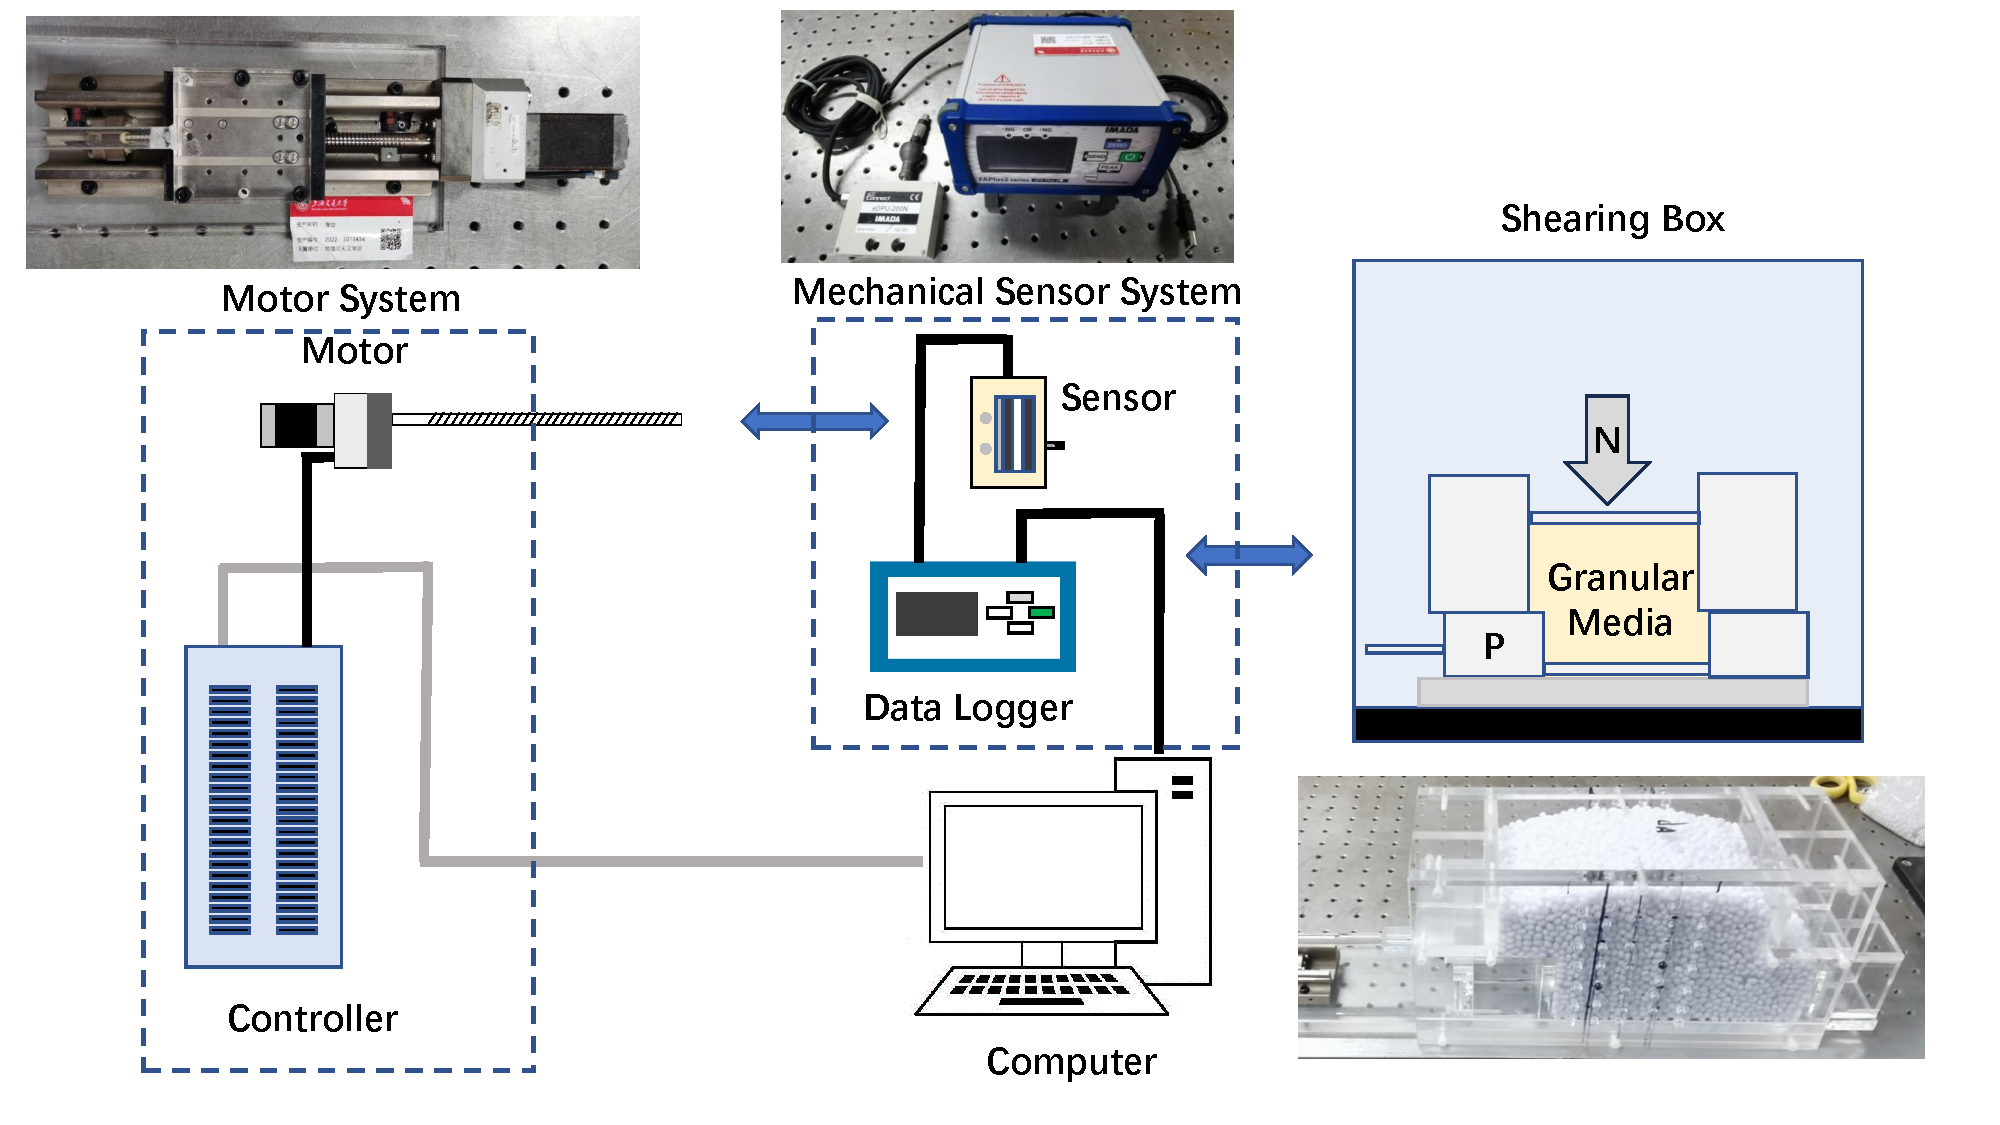
\includegraphics[height=8.5cm]{figures/4_apparatus.pdf}
    \bicaption{剪切装置与数据收集系统示意图}{Schematic diagram of the shearing apparatus and data collection system}
    \label{fig:apparatus_2}
  \end{figure}

接下来我们来介绍各部件的主要功能:

\begin{enumerate}
    \item 骏河步进电机。通过连杆与剪切盒的活塞部分固定连接,从而推动其进行对颗粒介质的剪切。电机通过 D214-2-2ek 信号线连接至控制器,控制器通过 USB 信道连接至计算机。计算机通过 DSCONTROL-WIN 软件来对电机进行控制,可以控制电机的运动方式为连续/步进,电机旋转方向和速度等参数。
    \item IMADA 力学传感系统。由 Sensor 和 Data Logger 两部分组成,Sensor 通过信号线将感受的力大小传递至 Data Logger;后者通过 USB 信道将数据实时传递至计算机,通过 Force Recorder 软件读取数据,力学传感器的最高采集频率为 2000 \unit{\hertz},力的分辨率则是 0.1 \unit{\newton}。在所需数据记录完毕后,即可通过 .csv 格式导出以供数据分析。
    \item 剪切盒。材质和单轴应力容器所使用的材质一样,是由亚克力板制作的,原本用于 X 光辐照探测剪切带。在未剪切时,其内部容积为 $18\times 10\times 12$ $\unit{\centi\meter}^{3}$ 的立方体,受电机控制的横截面积为 $10\times 6$ $\unit{\centi\meter}^{2}$ 的活塞带动固连的底板进行推动,而所推动的活塞截面的高度小于颗粒介质的高度而对颗粒介质有剪切作用。由于剪切盒的活塞在运动方向上存在长度上限,为了避免颗粒漏出剪切盒的剪切应变也存在上限。剪切盒的封顶板可以拆下而替换为施加应力的活塞板,从而检测不同堆积方式的颗粒介质的力学响应机制。
\end{enumerate}

\section{应力-应变曲线}

\subsection{RCP 与 RLP 的剪切响应差异}

我们使用同一剪切装置,在未施加应力与施加应力 P = 3.97 \unit{\kilo\pascal} 下分别测定 6 \unit{\milli\meter} ABS 球所组成的颗粒介质的应力-应变曲线。为了充分展现颗粒介质的滞滑特性,我们在实验时设定的剪切速率极低;在 DSCONTROL-WIN 软件上设定的剪切速率为 20 \unit{pps},对应于现实世界的剪切速度约为 $60\sim 70$ \unit{\micro\meter}/\unit{\second}。图~\ref{fig:shearstress} 展示了以上两种堆积在相同剪切速率下的剪切应力-应变曲线,其中定义域分别为剪切位移和时间。

\begin{figure}[htbp]
	\centering
	\bisubcaptionbox{随机松散堆积的剪切应力-应变曲线}%
                  {Shear stress-strain curves for random loose packing}%
                  [15cm]{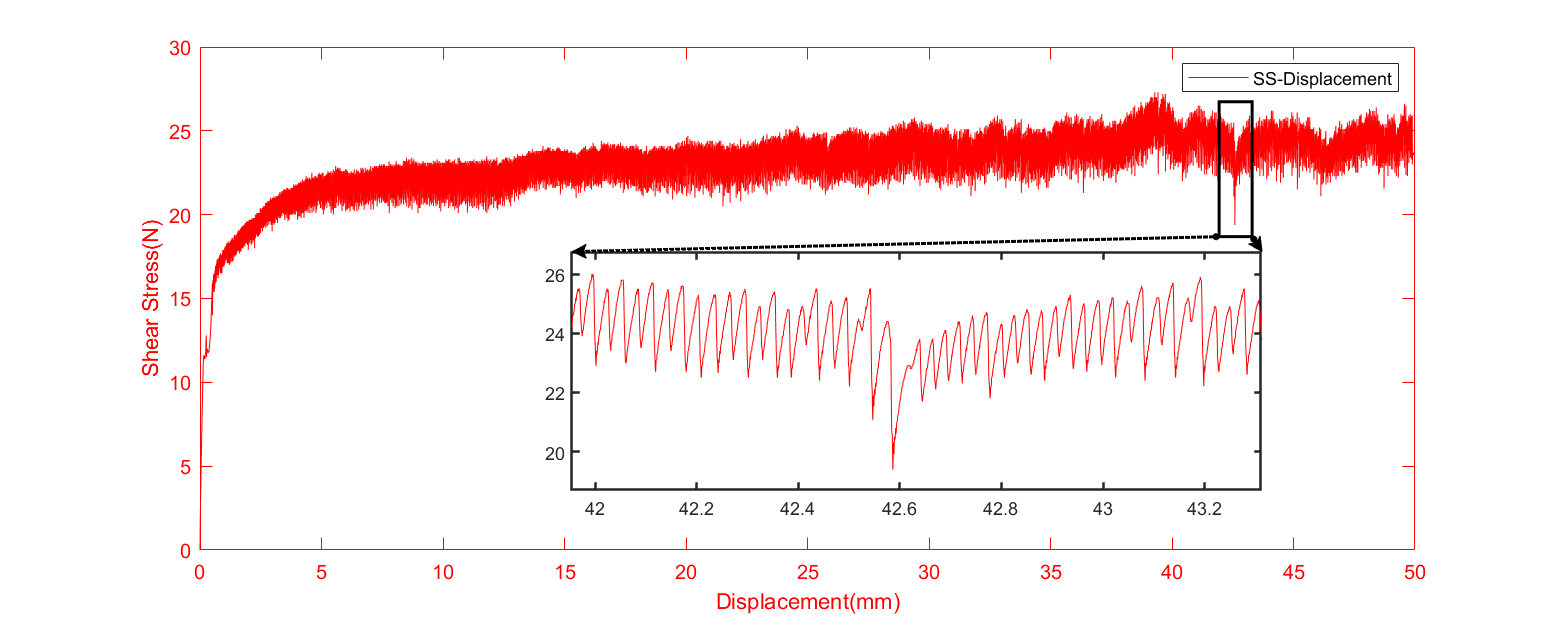
\includegraphics[width=1\linewidth]{4_shearstress_displacement.png}}\\
  \bisubcaptionbox{随机密集堆积的剪切应力时域曲线}%
                  {Shear stress in time domain for random close packing}%
                  [15cm]{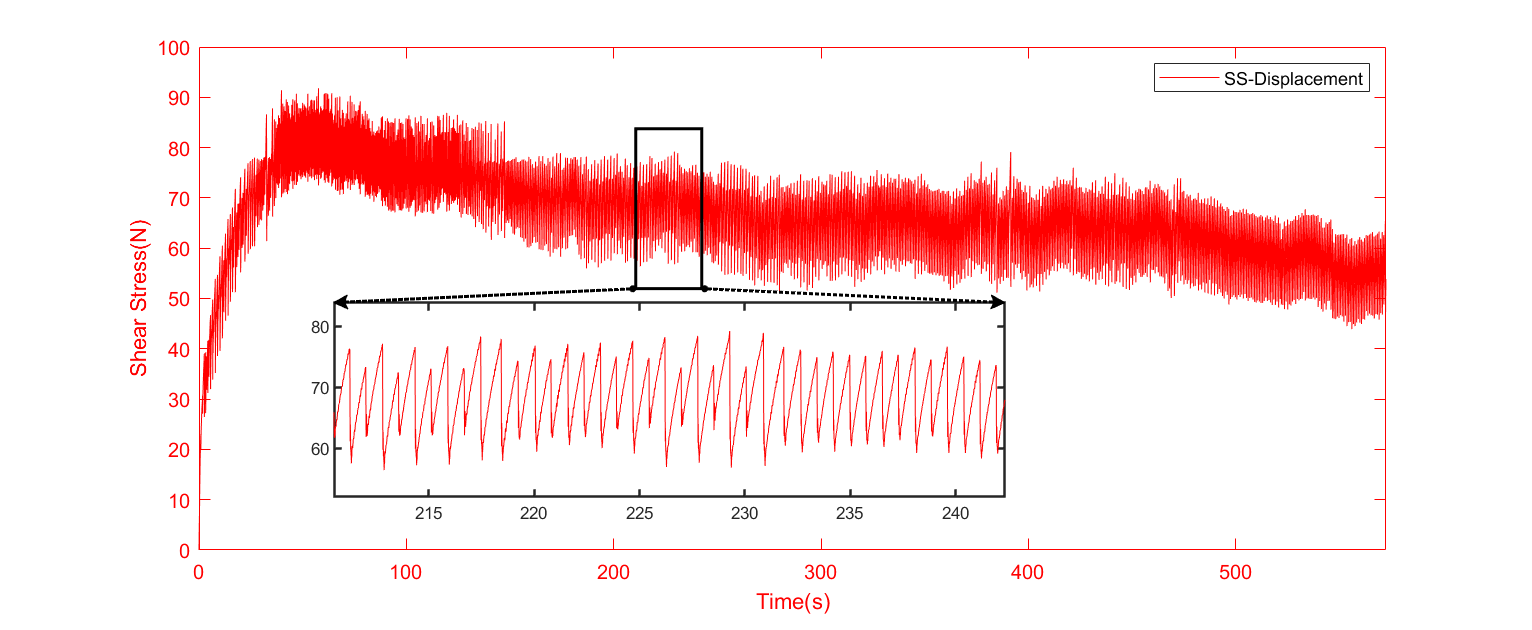
\includegraphics[width=1\linewidth]{4_shearstress_time.png}}
  \bicaption{RLP 与 RCP 在剪切速率为 20 pps 下的力学响应曲线}{Mechanical response curves of RLP and RCP at shear rate of 20 pps}\label{fig:shearstress}
\end{figure}

\subsection{蠕变与滞滑}

在 RCP 中得到的应力曲线更接近于传统的固体材料,即分为弹性区、屈服区(yielding state)和临界区(critical state)。

\begin{itemize}
  \item 弹性区。在剪切位移较小时,大部分颗粒位置几乎不变,而只是存在着较小程度的挤压和摩擦,这种接近线性的应力-应变关系和弹性行为相似,即产生蠕变现象;
  \item 屈服区。当剪切位移增大到一定程度时,即颗粒间的相互摩擦开始接近静摩擦阈值,颗粒开始产生相对滑动、重排,并且这种过程是不可逆的。应力的最高点即为颗粒介质的屈服强度。从放大图像观察可知,出现了剪切应力的反复积累提升、骤降的现象,这种过程伴随着频繁的力链断裂和重构,即滞滑。
  \item 临界区。在剪切位移进一步增大时,此时颗粒介质展现出可被类比于固-液相变的性质,即颗粒介质在外部剪切的激励下出现了流动的现象。
\end{itemize}

我们可以按照应力降(Shear Stress Drop,SSD)的大小来对滞滑事件进行粗分类。类比于环形剪切相关实验中的方法,我们按照应力降的幅值将滞滑事件分为三类:微滞滑(micro-,$\text{SSD}<0.2$ \unit{\newton})、小滞滑(minor-,0.2 \unit{\newton}$<\text{SSD}<0.4$ \unit{\newton})和主滞滑(major-,在地震学也被称作 failure,$\text{SSD}>0.4$ \unit{\newton})。

\section{本章小结}